\documentclass{article}
\usepackage[utf8]{inputenc}
\usepackage[T2A]{fontenc}
\usepackage[russian]{babel}
\usepackage{amsmath}
\usepackage{graphicx}

\begin{document}

\title{Практика 2}
\author{Ращупкин Е, Боков Е, Мишунин Н}
\maketitle

\section{Задача 1}
Интерфейс доступа к коллекции элементов Collection обобщает интерфейс работы со списками List. Абстрактный класс BaseCollection реализует интерфейс Collection, абстрактный класс BaseList является потомком BaseCollection и реализует интерфейс List, оставляя операции по хранению данных дочерним классам.

\begin{itemize}
    \item Используя наследование, добавьте в модель класс ArrayList, реализующий операции со списками с помощью массива.
    \item Пусть интерфейс List содержит операцию get получения элемента списка с заданной позицией k. Укажите, в каких классах должна быть объявлена данная операция, чтобы модель была согласованной. Ответ поясните.
    \item Пусть интерфейс Collection содержит операцию add добавления элемента obj. Укажите, в пространстве имен каких классов может присутствовать поведение, реализующее операцию add. Ответ поясните.
\end{itemize}

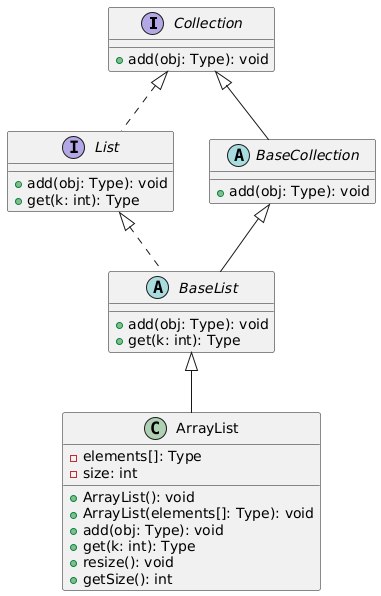
\includegraphics[width=\textwidth]{1.png}
\section{Задача 2}
Класс Collections содержит общедоступную статическую операцию addAll c возвращаемым значением типа Boolean. Первый параметр операции называется coll и имеет тип collection, второй параметр называется elements и имеет тип object и кратность больше нуля.

\begin{itemize}
    \item Добавьте в класс Collections статический атрибут empty типа Collection, предназначенный только для чтения.
    \item Добавьте в класс черту поведения, которая реализует операцию addAll.
\end{itemize}

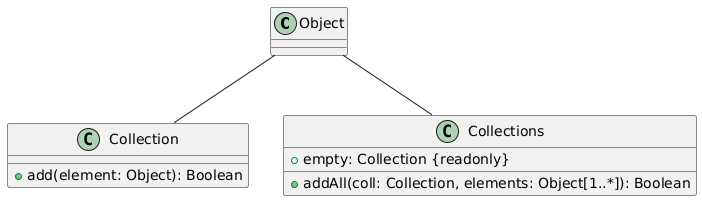
\includegraphics[width=\textwidth]{2.png}

\section{Задача 3}
На рис. представлены шаблонные интерфейсы Map и Entry. Интерфейс Map позволяет по ключу типа К получить значение типа V. Интерфейс Entry представляет собой пару значений.

\begin{itemize}
    \item Измените модель так, чтобы шаблон Entry использовал параметры шаблона Map.
    \item Определите интерфейс Map\_StringInteger, который указывает String типом ключа и Integer типом значения в шаблоне Map.
    \item Сколько операций содержит интерфейс Map\_StringInteger? Ответ поясните.
\end{itemize}

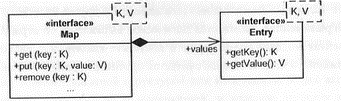
\includegraphics[width=\textwidth]{task3.png}

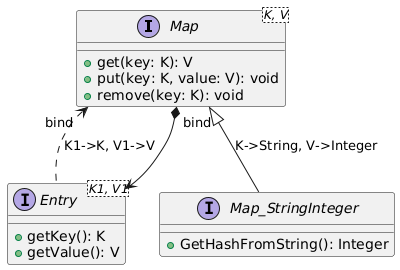
\includegraphics[width=\textwidth]{3.png}

\section{Задача 4}
Интерфейс работы с ассоциативным массивом Map в своем пространстве имен содержит интерфейс работы с элементом массива Entry. При этом реализации интерфейса Map включают несколько реализаций интерфейса Entry.




\begin{itemize}
    \item Добавьте в модель класс HashMap, реализующий ассоциативный массив с помощью хэш-таблицы, и класс HashEntry, реализующий интерфейс работы с элементом массива.
    \item Пусть в классе HashMap определена частная операция увеличения размера resize. При каких условиях данная операция будет доступна классу HashEntry?
    \item Используя шаблоны, укажите, что тип ключа и тип значения интерфейса ассоциативного массива должны совпадать с типов ключа и типом значения в интерфейсе работы с элементов массива.
\end{itemize}

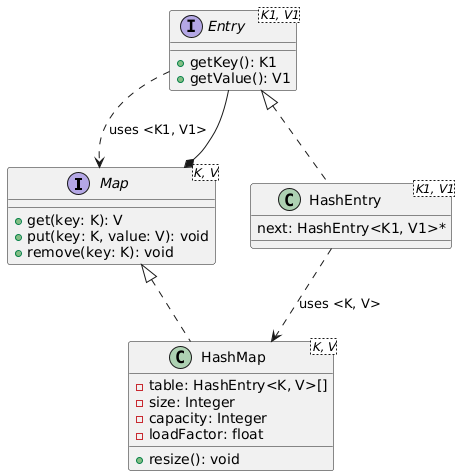
\includegraphics[width=\textwidth]{4.png}

\section{Задача 5}
Узел дерева Node может иметь несколько дочерних child узлов того же класса Node.

\begin{itemize}
    \item Используя модель, приведите пример бинарного дерева, состоящего из семи узлов Node.
    \item Постройте модель дерева, в котором каждый узел имеет от двух до пяти дочерних узлов.
    \item Разработайте модель дерева, узлы которого могут быть двух видов: узел Oden и узел Enod.
\end{itemize}

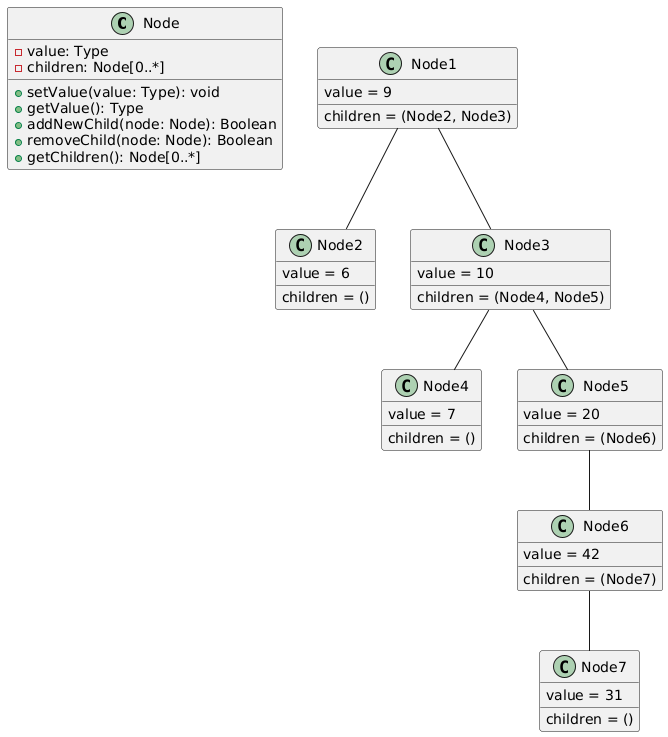
\includegraphics[width=\textwidth]{5.png}

\section{Задача 6}
Диск Disk содержит несколько папок Folder которые могут содержать файлы File и папки. Произведения Content хранятся на дисках несколькими файлами.

\begin{itemize}
    \item Используя классы ассоциаций, постройте модель хранения произведений на дисках.
    \item Дополните модель, укажите, что произведение может быть либо картиной Picture, либо музыкой Music, либо фильмом Movie.
    \item Может ли произведение храниться на одном диске в разных файлах? Ответ поясните.
\end{itemize}

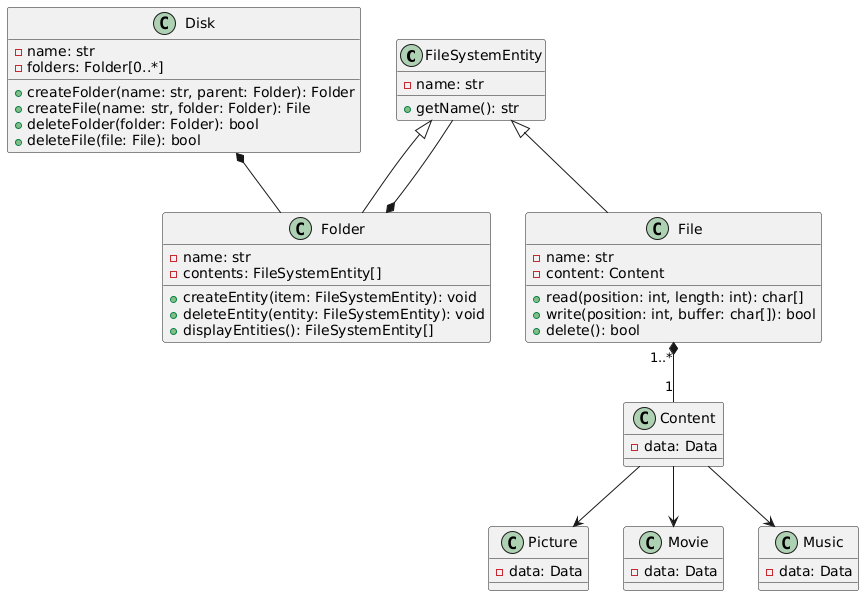
\includegraphics[width=\textwidth]{6_1.png}
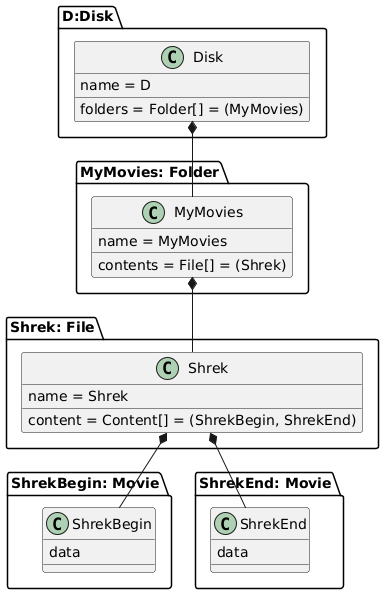
\includegraphics[width=\textwidth]{6_2.png}

\section{Задача 7}
Каждый экземпляр абстрактного класса контроллер Controller связан по ассоциации Sensor с несколькими датчиками поезда TrainSensor. В ассоциации контроллер играет роль управляющего controller. Датчик поезда участвует в ассоциации как датчик sensor с частной видимостью.

\begin{itemize}
    \item Используя квалификаторы, укажите, что каждому значению индекса index типа String соответствовало не более одного датчика в ассоциации Sensor.
    \item Уточните класс контроллера, укажите, что класс принимает сигналы приближения поезда TrainSpotted и отдаления поезда TrainLeft, имеет общедоступную операцию выполнения команд execute с параметром cmd типа данных Command и возвращает значение типа данных Result.
    \item Определите класс цифрового контроллера DigitalController, уточняющий класс контроллера. В классе цифрового контроллера определена операция executeDigital, которая переопределяет операцию выполнения команд контроллера и возвращает цифровой результат DigitalResult.
    \item Используя экземпляры классов, приведите пример контроллера с двумя датчиками.
\end{itemize}

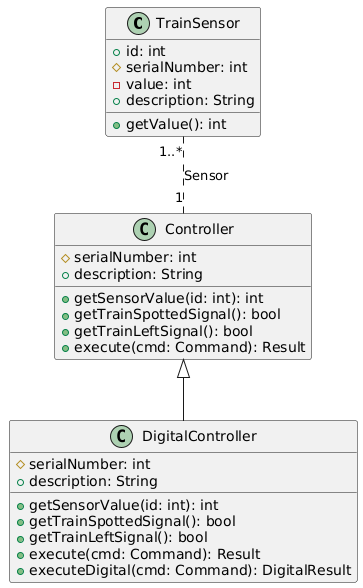
\includegraphics[width=\textwidth]{7.png}

\section{Задача 8}
В файловой системе данные сохраняются в цепочках кластеров, записанных в таблице размещения файлов FAT. Таблица содержит кластеры Cluster, при этом кластер является индексом следующего кластера в цепочке. Кластер директории Folder содержит lists (упорядоченный набор записей Entry о файлах и директориях). Каждая из записей указывает размер size, имя name, атрибуты attrs и начальный кластер Cluster.

\begin{itemize}
    \item Уточните модель, укажите, что у кластера может не быть следующего в таблице размещения файлов.
    \item Используя ограничения, определите тип данных целое Byte с диапазоном значений от 0 до 255.
    \item Добавьте новый вид кластера – кластер данных Data, содержащий данные файлов. Операция getData позволяет получить данные класса в виде массива с элементами типа Byte.
    \item Укажите, что кроме Folder и Data кластеры бывают только испорченными Bad и резервными Reserved. 
    \item Приведите пример таблицы размещения файлов на пять кластеров с одной директорией folder и двумя файлами file1 и file2. File1 размещен в кластере с номером 3, file2 – в кластерах 2 и 4. Таблица размещается в первом кластере, он резервный.
\end{itemize}

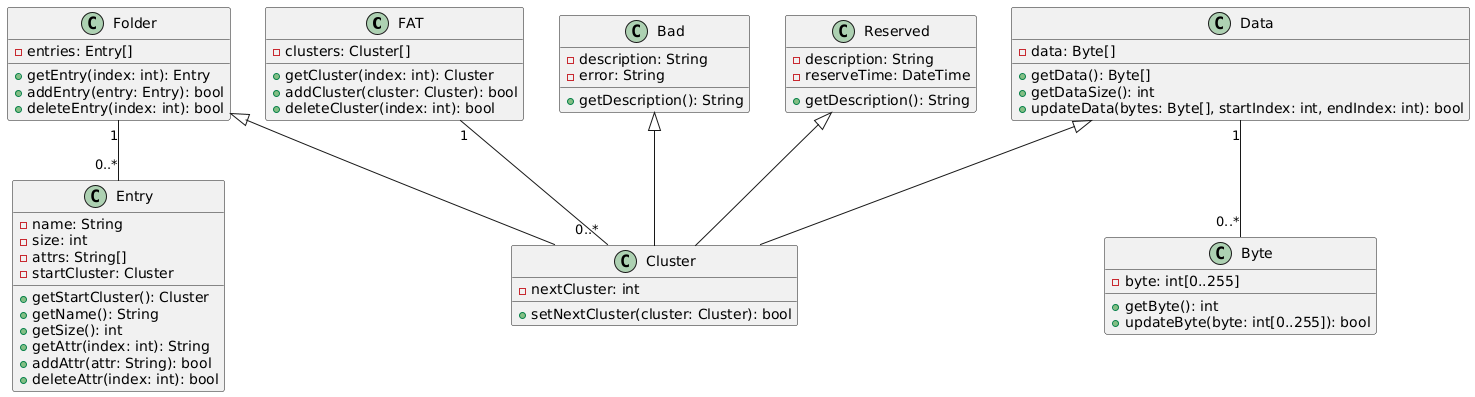
\includegraphics[width=\textwidth]{8.png}
\end{document}
